\onehalfspacing
% \chapter{Literature Review}
% \label{chapter:literature}

%%% SECTION
% \section{Literature Review}
\section{Foundations}

The overexpression of Cyclin D1 in human cancer is well-known\cite{Lamb2003} and has been reported in several studies\cite{2017Reena}.
An interesting recent work conducted by Albero et al.\cite{10.1172/JCI96520}, focuses on the study of this overexpression and how it produces a global trancriptional donwmodulation in lymphoid neoplasms. In their own words:

"This finding of global transcriptional dysregulation expands the known functions of oncogenic Cyclin D1 and suggests the therapeutic potential of targeting the transcriptional machinery in Cyclin D1–overexpressing tumors."
\cite{10.1172/JCI96520}

Studies like the one performed by Mohanty et al.\cite{Mohanty2017} show the importance of Cyclin D1 (CCND1) in the maintenance of MCL tumor cell lines, but leave unclear the protective role of this gene in preventing DNA damage during replication in MCL. This mentioned study point out some conflicts with another study on CCND1 performed by Klier et al.\cite{Klier2008}, which reports that silencing CCND1 in MCL for up to seven days cause growth arrest but not cell death in MCL.\cite{Mohanty2017}.

Another interesting study performed by Tiemann et al.\cite{Tiemann2011} demonstrate how targeting Cyclin D1 and Cyclin D2 in chemotherapy can lead to enhance the efficacy of chemotherapy agents.

The above cited studies are a small set of examples on how important it is to increase the knowledge of the transcriptional function of Cyclin D1 in order to improve the prevention and treatment of MCL.

In parallel, other studies \cite{DiSante2017} \cite{Casimiro2016}, have shown the role of Cyclin D1 in the cell cycle and its influence in the DNA-damage repair process.

In addition to the already commented works, the field of Artificial Intelligence and in particular the Machine Learning discipline inside of it, has been winning attention in many fields, being medicine one of them.
Machine Learning has been widely used to study different types of cancer, and some examples of it will be provided in the following section.
As a result, Machine Learning has been added to the pipeline of biological studies and, among other important consequences, it has produced a big impact improving the identification of discriminant pathways, as shown in the study done by Barla et a.\cite{Barla2014}.

Another foundation for this project is the Gene Set Enrichment Analysis method (GSEA) \cite{Subramanian15545} which was presented in 2005.
GSEA has had a big impact in the statistical analysis of gene sets, prove of that is its more than 10000 citations.
GSEA is an analytical method that allows the researchers to focus on gene sets instead of individual genes, as it was done before.
Thanks to that, it enables the detection of biological processes like metabolic pathways, transcriptional programs or stress responses. 
Apart from being a statistical analysis method, it also provides a software package and a database composed by more than 1000 gene sets that facilitates its usage and experimentation.

Although the intention of this text is not to provide an exhaustive explanation of how GSEA works, it is important to offer a minimum introduction to the method, to be able to understand better the way how Machine Learning can improve it.

A basic schema about how GSEA works is described in the following figure:

\begin{figure}[h]
    \centering
    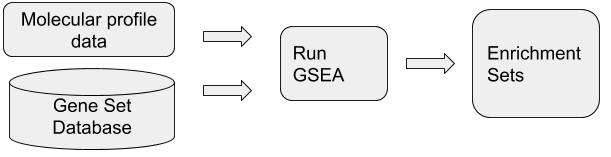
\includegraphics[scale=0.5]{../figs/GSEA_schema.png}
    \caption{GSEA Schema.}
    \label{fig:gsea-sch}
\end{figure}

GSEA receives two inputs, a molecular profile data and a Gene Set Database. Using this two inputs, GSEA will calculate an Enrichment Score (ES) between phenotypes for each gene contained in the molecular profile.
Thanks to this ES, GSEA will be able to identify which set of genes offers statistical significance and will make possible the identification of biological processes.

Due to the big amount of data, in terms of genes, that this kind of analysis can face, it is really important to make a good selection of them beforehand. This is one of the situations where Machine Learning is able to help, providing Feature Selection algorithms that can optimize the genes selected to be passed as an input to the GSEA method.

In relation with that methodology, it is also interesting to remark the importance of choosing a proper metric for the ranking of genes, as shown in the work carried out by Zyla et al.\cite{Zyla2017}.

All the above concepts have acted as a foundation to trigger the main ideas behind the objectives of the project presented here.

\section{Similar Work}

As commented before, it is easy to find examples of the usage of Machine Learning in the field of cancer study. It has been widely used for different purposes such as classification\cite{Chuang2007} and prediction of tumors, treatment prediction, and also to boost the performance of the biological analysis pipelines using techniques like feature selection\cite{SINGH201552}\cite{Bashiri2017}.

An interesting example is found in the study conducted by Ten et al.\cite{Tan2018} where Machine Learning techniques were introduced in their pipeline in order to improve the analysis of multiple gene expression profiles in cervical cancer.
A particular important fact extracted from that article, is that previous studies were focused either in statistical analysis methods or Machine Learning methods, but that one integrates both methodologies for the meta-analysis, which is also one of the objectives pursued by this work.

Another similar interesting work is found in the study elaborated by Park et al.\cite{Park2018}. In there, the identification of disease-related genes and disease mechanism is investigated using Machine Learning techniques. The study presents a novel method for gene-gene interaction (GGI) based on the usage of the Random Forest algorithm. This method is suitable for the discovery of significant GGI from heterogeneous gene expression datasets, and has the potential to be used in the research of different disease groups.

\section{Ongoing and Future Projects}

Several studies\cite{Inamdar2016}\cite{Steiner2018}\cite{Schieber2018}\cite{Dreyling2016} agree on the necessity of the development of more personalized (patient-centric) treatments. Such treatments will be possible through an evaluation of each patient unique set of genomic complications and will result in more accurate treatments that will be highly effective and will not over-treat the patient. Is also important to comment that together with personalized treatments, more reliable predictive tools to improve the prognostic of each patient need to be developed, but before this point will be reached, new biomarkers and pathways that will enhance the understanding of MCL need to be discovered. This is an active area of study and it is also one of the purposes of the work presented here.

Apart from the ongoing studies on MCL, it is worth to mention that the field of Artificial Intelligence continues its expansion. Every day, new studies, methods and developments are performed. As a consequence, more fields are adopting Artificial Intelligence approaches to improve their results. Of course, medical research is also profiting from all the consequent research and development.
This Artificial Intelligence explosion has the potential to change drastically the way a scientific research will be done in the future, as a small example of it, new ways of knowledge discovery (cognitive discovery) are studied and developed, combining different areas of Artificial Intelligence like Knowledge Graphs, Natural Language Processing, Semantic Search, etc. The products obtained from that work will help the future researchers to find remarkable literature during the literature review that takes place at the starting phase of a scientific research.\cite{Raymond2019}